\documentclass[letterpaper, 12pt]{article}
\usepackage[letterpaper, top=2.5cm, bottom=2.5cm, left=3cm, right=3cm]{geometry} %margenes
\usepackage[utf8]{inputenc} %manejo de caracteres especiales
\usepackage[spanish]{babel} %manejo de encabezados de inglés a español
\usepackage{fancyhdr} %formato de los encabezados de página
\usepackage{ragged2e} %alineado real justficado
\usepackage{graphicx} %manejo de imagenes
\usepackage{amsmath} %manejo de notación matemática
\usepackage{mathtools} %manejo de notación matemática
\usepackage{blindtext} %texto de relleno
\usepackage{cancel} %permite la simbolización de cancelación de terminos
\usepackage{enumitem}[shortlabels] %listas con letras
\usepackage{amssymb} %manejo de simbolog►1a matematica
\usepackage[titles]{tocloft} %manejo de elementos para el índice
\usepackage{float} %manejo de centrado para figuras
\usepackage{hyperref} %manejo d hipervínculos
\hypersetup{%formato de colors de hipervínculos, permite crear pdfs con enlaces a los temas
    colorlinks=true,      
    urlcolor=blue,
    linkcolor=blue
}
\pagestyle{fancy}
\fancyhf{}
\rfoot{\thepage}

\begin{document}
    
    %PORTADA
    \begin{titlepage}
        \begin{figure}[ht]
            \centering
            
\includegraphics[width=15cm]{logosITT.png}
        \end{figure}
        \centering
        {\scshape\LARGE Tecnológico Nacional de México\\Instituto Tecnológico de Tijuana\par}
        \vspace{1cm}
        {\scshape\Large Cálculo Diferencial\par}
        \vspace{1cm}
        {\scshape\Large Unidad 3\par}
        \vspace{1.5cm}
        {\huge\bfseries Límites y Continuidad\par}
        \vfill
        Asesor: \par
        C. Abraham Jhared Flores Azcona
        
        \vfill

        {\large \emph{``If it's close enough, it's good enough.''}}


    \end{titlepage}

    \newpage
    \thispagestyle{empty}
    \tableofcontents

    \newpage
    \pagestyle{fancy}
    \lhead{\textbf{Unidad 3: Límites y Continuidad}}
    \section{Noción del límite}
    \justify
    Existen tres tipos de noción: \emph{gráfica, numérica y analítica (se verá con mayor detalle)}. En estos siempre es importante la siguiente frase:
    \begin{center}
    \textbf{\emph{``If it's close enough, it's good enough''}.}  
    \end{center}
    \justify
    Todo esto es con el objetivo de determinar el comportamiento de una función cerca de un punto de interés, pero no realmente en ese punto.
    \\\newline
    De cajón decimos que si la función \(f(x)\) se acerca cada vez más a algún número \(L\) cuando los valores de \(x\) son mayores que \(a\) se aproximan cada vez más a \(a\), entonces \(L\) es el límite de 
    \(f(x)\) cuando \(x\) se aproxima por la derecha. Esto se representa así:
    \[\lim_{x\rightarrow a^+}f\,(x)=L\]
    Si la función \(f(x)\) se acerca cada vez más a algún número \(a\) cuando los valores de \(x\) \emph{que son menores que} \(a\) se aproximan cada vez más a \(a\) por la izquierda, entonces \(L\) es el límite
    de \(f(x)\) cuando \(x\) se aproxima a \(a\) por la izquierda. Esto se simboliza así:
    \[\lim_{x\rightarrow a^-}f\,(x)=L\]
    Las tres nociones principales consisten en lo siguiente:
    \\\newline
    \textbf{Numérico: }construye una tabulación como la siguiente:
    \\Ej: Calcular \(\lim_{x\rightarrow 2}f(x)\)
    \[\begin{matrix}
        x&1.9&1.99&1.999&1.9999&2&2.01&2.001&2.0001&2.00001\\
    f(x)&2.61&2.9601&2.996&2.9996&?&3.0401&3.004&3.0004&3.00004
    \end{matrix}\]
    Notese que por ambas direcciones, \(f(x)\) tiende a 3 por lo tanto \(\lim_{x\rightarrow 2}f(x)=3\)
    \\\newline
    \textbf{Gráfico: }determinar el límite a partir de la gráfica dada. Personalmente es la mejor noción.
    \\Ej: En base a la gráfica de \(f(x)\), calcular \(\lim_{x\rightarrow 2}f(x)\)
    \begin{figure}
        \centering
        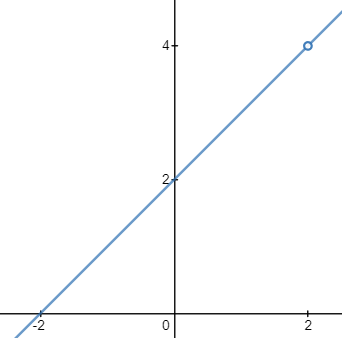
\includegraphics[width=8cm]{limite.PNG}
    \end{figure}
    De manera similar a casos anteriores, evaluamos por la izquierda y por la derecha, Vemos que en ambos, la gráfica se acerca a 3, por lo tanto \(\lim_{x\rightarrow 2}f(x)=3\)
    \section{Definición de límite de una función}
    Un límite existe si y solo si ambos límites laterales existen y son iguales.
    \[\lim_{x\rightarrow a}f(x)=L \leftrightarrow \lim_{x \rightarrow a^-}f(x)=\lim_{x \rightarrow a^+}f(x)=L\]
    Si quieren mas rigor, pueden buscar la definición \(\epsilon \delta\) del límite.
    \section{Propiedades de los límites}
    Como todo, las ``formulas'' que se pueden aplicar. Suponiendo que \(c\) es una constante, que \(\lim_{x\rightarrow a} f(x)=L_1\), y también que \(\lim_{x \rightarrow a} g(x)=L_2\). Entonces se tienen las siguietnes propiedades:
    \begin{itemize}
        \item \(\lim_{x \rightarrow a}\left(c\cdot f\,(x)\right)= c \cdot \lim_{x \rightarrow a}=cL_1\).
        \item Análogamente \(\lim_{x \rightarrow a} \left(c \cdot g\,(x)\right)=cL_2\).
        \item \(\lim_{x \rightarrow a}\left(f\,(x)\pm g\,(x)\right)=\lim_{x \rightarrow a}f\,(x)\pm \lim_{x \rightarrow a}g\,(x)=L_1 \pm L_2\).
        \item \(\lim_{x \rightarrow a}\left(f\,(x)\cdot g\,(x)\right)=\lim_{x \rightarrow a}f\,(x)\cdot \lim_{x \rightarrow a}g\,(x)=L_1\cdot L_2\).
        \item \(\lim_{x \rightarrow a}\frac{f\,(x)}{g\,(x)}=\frac{\lim_{x\rightarrow a}f\,(x)}{\lim_{x \rightarrow a}g\,(x)}=\frac{L_1}{L_2},\,\forall L_2\neq 0. L_1\neq 0 \land L_2=0\rightarrow \text{El límite no existe}\).
        \item \(\lim_{x \rightarrow a}\left(f\,(x)\right)^n=\left(\lim_{x \rightarrow a}f\,(x)\right)^n=L_1^n,\, \forall n\in \mathbb{Z}^+\).
    \end{itemize}
    \section{Cálculo de los límites}
    Más formulas y ejercicios... xd. Estos límites especiales son útiles al momento de calcular los mismos.
    \\\newline
    \textbf{Límite de una función constante:}
    Para cualquier constante \(c\) y cualquier número real \(a\):
    \[\lim_{x\rightarrow a}c=c\]
    \textbf{Límite de la función \(f(x)=x\):}
    Para cualquier número real \(a\):
    \[\lim_{x \rightarrow a}x=a\]
    \textbf{Límite de una potencia:}
    Este límite se desprende de las propiedades ya enunciadas:
    \[\lim_{x \rightarrow a}x^n=a^n\]
    donde \(n\) es cualquier entero mayor que cero y \(a\) es cualquier número real.
    \\\newline
    \textbf{Límite de un polinomio:}
    Para cualquier \(P(x)\) que es un polinomio y \(a\) es cualquier número real.
    \[\lim_{x\rightarrow a}P(x)=P(a)\]
    \textbf{Límite en una función racional:}
    Supongamos que \(\lim_{x \rightarrow a}f(x)=L\) y que \(n\) es cualquier entero mayor que cero y diferente 1; entonces:
    \[\lim_{x \rightarrow a}\sqrt[n]{f(x)}=\sqrt[n]{\lim_{x \rightarrow a}f(x)}=\sqrt[n]{L}\]
    Si \(n\) es un número par, se supone que \(L\) es mayor que cero; si no es así, el límite no existe.
    \\\newline
    \textbf{Límite de un cociente de funciones:}
    \begin{itemize}
        \item \(\lim_{x\rightarrow a}\frac{p(x)}{q(x)}=\frac{L_1}{L_2}\), siempre que \(L_2\neq 0\).
        \item Si \(\lim_{x \rightarrow a}f(x)=0\) y \(\lim_{x \rightarrow a}g(x)=0\), entonces \(p(x)\) y \(g(x)\) son divisibles entre \((x-a)\).
        \item Si \(\lim_{x \rightarrow a}f(x)\neq 0\) y \(\lim_{x \rightarrow a}g(x)=0\), entonces \(a\) es un polo de ese cociente y por ende \emph{el límite no existe}.
    \end{itemize}
    \section{Límites laterales}
    Literalmente es evaluar los límites por la izquierda y la derecha, lo cual ya se tocó en temas anteriores.
    \section{Límites infinitos y límites al infinito}
    Existen ocasiones en las cuales nos preguntan acerca del comportamiento de estos Límites. Los límites infinitos son el tipo de límites en los que \(f(x)\) crece o decrece sin cota (infinitamente) cuando \(x\) tiende a un número \(a\). Los límites al infinito son cuando evaluamos
    dicho límite en el infinito. Un ejemplo trillado pero muy ilustrativo es el de \(f(x)=\frac{1}{x}\):
    \begin{figure}[H]
        \centering
        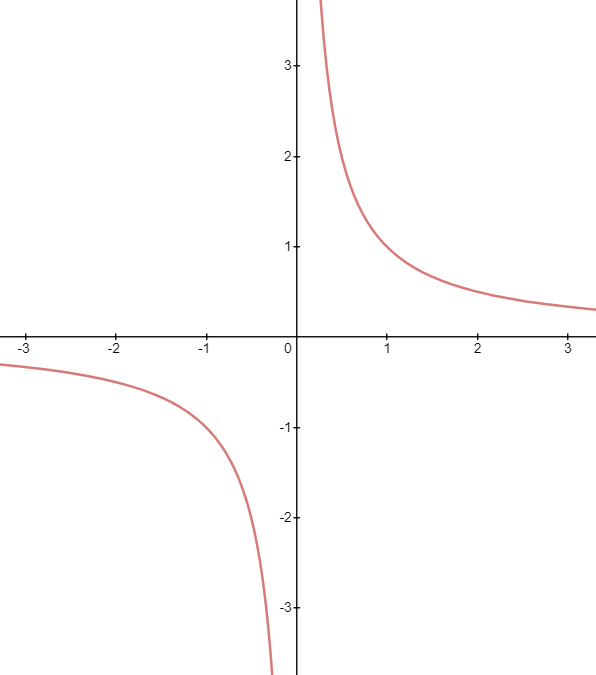
\includegraphics[width=10cm]{unosobrex.PNG}
        \caption{Gráfica de \(f(x)=\frac{1}{x}\)}
    \end{figure}
    La razón analítica del porque dicha función nos da una indeterminación al dividir entre 0 es porque:
    \[\lim_{x\rightarrow 0^-}\frac{1}{x}\neq \lim_{x\rightarrow 0^+}\frac{1}{x}\]
    O descrito en palabras humanas, el límite por la derecha se dispara al infinito positivo y el de la izquiera hacia el infinito negativo, por ende los límites no coinciden por sus evaluaciones laterales y dicho límite no existe.
    \\\newline
    Para el caso de los límites en el infinito, ahora evaluamos a la función cuando esta tiende al infinito, escrito de manera simbolica:
    \[\lim_{x \rightarrow \infty}f(x)\]
    Su resolución generalmente revolvera en el tipo de funciones de tipo polinomial que componen a la división de dos funciones, una forma representativa sería la siguiente:
    \[\lim_{x \rightarrow \infty}\frac{a_1x^n+a_2x^{n-1}+\dots+a_0}{b_1x^m+b_2x^{m-1}+\dots+b_0}\]
    Donde dicho limite es igual a:
    \[\text{• }\frac{a_1}{b_1}\text{ si }n=m;\, \text{ • }0\text{ si }n<m;\, \text{ • No existe si }n>m;\]
    \section{Asíntotas}
    Definida como una linea recta prolongada infinitamente que se acerca progresivamente a una curva sin nuna llegar a tocarla. Por lo visto en temas anteriores, volvemos a aplicar
    las evaluaciones de los límites infinitos y los límites en el infinito para los cocientes de funciones polinomiales.
    \subsection*{Asíntota vertical}
    Se obtiene de la siguiente manera:
    \[\lim_{x\rightarrow a} \frac{p(x)}{g(x)}=\text{No existe}\]
    Con ello se considera que \(x=a\) es el valor absciso donde se encuentra dicha linea recta vertical.
    \subsection*{Asíntota horizontal}
    Se obtiene de la siguiente manera:
    \[\lim_{x \rightarrow a}\frac{p(x)}{q(x)}=\frac{L_1}{L_2},\,\forall L_2\neq 0\]
    Se considera que \(y=\frac{L_1}{L_2}\) es la ecuación de la linea recta horizontal.
    \section{Continuidad en un punto y en un intervalo}
    Simplemente es saber si la función no está mocha en algun punto o en un intervalo. Para fines prácticos, se considera que una función \(f\) escontinua en \(x=a\) cuando:
    \begin{itemize}
        \item \(f(a)\) está definida.
        \item \(\lim_{x\rightarrow a}f(x)\) existe.
        \item \(\lim_{x\rightarrow a}f(x)=f(a)\).
    \end{itemize}
    Hay que estár muy atentos a las gráficas llegara el caso que se necesite hacer el análisis gráfico. Si nos piden evaluar en un intervalo, evaluamos los extremos de dicho intervalo, recalco que
    dependiendo del tipo de comportamiento de la función, dependera mucho su continuidad.
    \section{Tipos de discontinuidades}
    Generalmente, cualquier punto donde la gráfica esté mocha se considera discontinuo.
    \section*{Hipervínculos de material complementario:}
    \addcontentsline{toc}{section}{Hipervínculos de material complementario:}
    El acceso es CON CORREO INSTITUCIONAL.
    \begin{itemize}
        \item \href{https://docs.google.com/document/d/1mhFr7S5rJ7TwR297Kd6l8b6NPvYkUAlpWIxuz4VKV2w/edit?usp=sharing}{\textbf{Pizarras Online de Miro (compendio de los enlaces).}}
        \item \href{https://drive.google.com/drive/folders/1yL1gAIbVpgKB3h8498KFNE7NDZjoxIWa?usp=sharing}{\textbf{Carpeta de los Documentos PDF.}}
        \item \href{https://drive.google.com/drive/folders/1TPtNSe4ErSgaBLw2kgYDQadyXqvh6AYC?usp=sharing}{\textbf{Grabaciones de las asesorías y demás.}}
    \end{itemize}

\end{document}